\chapter{轨迹替换、混合高斯噪声层和仿真时间奖励}
本章介绍了在TD3算法和事后经验重放基础上,针对开放任务特点进行的几个改进。
其中轨迹替换方法很好地解决了事后经验重放中的未来替换方法难以应用于状态变量互相耦合,难以区分已完成的目标和期望目标的开放任务的问题。
混合高斯噪声层是在固定大小的随机探索噪声基础上的改进,目的是为了使智能体获得更好的随机探索策略,避免收敛到局部最优的策略上。
仿真时间奖励作为一种与特定任务无关的内部奖励,可以用于提升探索效率,加速含有稀疏奖励的开放任务的学习进程;也可以用于在未获得任务相关的奖励时,使智能体在环境中探索并学习元探索策略。
\section{轨迹替换方法}

在Gym环境中进行初步实验时,与\ref{HERsec}中的替换方法不同,不在采样时对已完成的目标进行替换,而是在将新的迁移保存到重放缓冲中时对整个片段进行替换,并把未替换和替换后的轨迹都加入到重放缓冲中。
换句话说,每当一个片段结束时,对这个片段中由所有迁移构成的整个轨迹中的已完成的目标进行替换,并把替换后的一整个新轨迹添加到原轨迹之后。

形式化地,轨迹替换会从重放缓冲中取出一整个轨迹的副本$s[1:T]=(o[1:T], g^a[1:T], g^d[1:T])$,并对其做如下替换:
$$g^d[1:T]=g^a[-1]$$
$$r[1:T]=reward(g^d[1:T], g^a[1:T])$$
并将所替换后的轨迹添加到重放缓冲中。
其中$s[1:T]$表示从$t=1$到$t=T$的状态向量序列$s_1, s_2, \cdots, s_T$。

如算法\ref{trajrepl}所示,在得到轨迹中的一个迁移$(s_t,a_t,r_t,s_{t+1})$后,首先将状态$s_t$分解为$(o_t, g^a_t,g^d_t)$,其中$o_t$是环境观测量,$g^a_t$是已完成的目标,$g^d_t$是期望目标。
然后使用$T$时刻的已完成目标将其余状态中的期望目标替换掉,并使用奖励函数$reward$重新计算奖励。
使用此方法获得的替换后的轨迹会和原轨迹一起放入重放缓冲中并被用于训练演员网络和评论家网络。
\begin{algorithm}
    \AlgoBiCaption{轨迹替换方法\label{trajrepl}}{Trajectory Replacement Strategy}
    \KwIn{替换前的轨迹$(s_t, a_t, r_t, s_{t+1}), t=1, 2, \cdots, T$}
    \KwOut{替换后的轨迹$(s'_t, a_t, r'_t, s'_{t+1}), t=1, 2, \cdots, T$}%

$(o_T, g^a_T, g^d_T) = s_T$\\
\For{$t$=1 to $T$}
{
    $(o_t, g^a_t, g^d_t) = s_t$\\
    $s'_t=(o_t, g^a_t, g^a_T)$\\
    $(o_{t+1}, g^a_{t+1}, g^d_{t+1}) = s_{t+1}$\\
    $s'_{t+1}=(o_{t+1}, g^a_{t+1}, g^a_T)$\\
    $r'_t=reward(g^a_T, g^a_t)$
 }
    
\end{algorithm}

实验在\ref{gymexp}中设计的系统中进行,使用的实验参数见表\ref{pretable}。
    \begin{table}[htbp]
        \caption{初步实验参数}
        \label{pretable}
    \vspace{0.5em}\centering\wuhao
    \begin{tabular}{ccccc}
    \toprule[1.5pt]
    实验参数 & 值\\
    \midrule[1pt]
        $\epsilon_{noise}$ & 0.2\\
        $\sigma_{clip}$ & 0.5\\
        $M$ & 5120\\
        $\epsilon_{rand}$ & 0.3\\
        $\gamma$ & 0.99\\
        $\alpha$ & $3\times 10^{-4}$\\
        $B$ & 8\\
        $\tau$ & 0.005\\
        $T$ & 50\\
        $f_\mu$ & 2\\
        $T_{start}$ & $2.5\times 10^4$\\
        $N_{sample}$ & 10 \\
    \bottomrule[1.5pt]
    \end{tabular}
    \end{table}
    其中$\epsilon_{noise}$是在更新评论家网络权重,使用靶演员网络计算动作向量时添加进去的高斯噪声的标准差,$\sigma_{clip}$是对此噪声进行裁剪的阈值,裁剪后有噪声大小在区间$[-\sigma_{clip},\sigma_{clip}]$以内。
    $M$是重放缓冲能保存的迁移的最多数量。
    $\epsilon_{rand}$是采用$\epsilon$-greedy探索方法进行探索时,随机采样动作的概率大小。
    $\alpha$是演员网络和评论家网络的优化器的学习率。
    $B$是从重放缓冲中采样迁移的批次大小。
    $\tau$是\ref{td3sec}中所述的指数滑动平均系数,在实验中发现,$\tau$的值应保证在10个片段之后原靶网络权重所占比例在10\%左右较好,即$(1-\tau)^{10T}\approx 10\%$。
    $T$是每个片段的最大时间步数。
    $\gamma$是前述折扣系数,在实验中发现,$\gamma=1-\frac{1}{T}$是较好的值,因此在实验中使用的$\gamma$值是在$1-\frac{1}{T}$基础上微调得到的。
    每经过$f_\mu$个时间步,才对演员网络权重进行更新一次,而评论家网络每权重更新和对靶网络权重的指数滑动平均更新在每个时间步都要做。
    在$t<T_{start}$时,使用完全随机的采样来得到智能体要做的动作,在$t\geq T_{start}$时,才开始使用演员网络获取动作向量。
    每经过$N_{sample}$个片段记为一代(epoch),对损失、奖励和成功率进行统计,最后绘制关于代的曲线图。

        \begin{figure}[htpb]
        \centering
        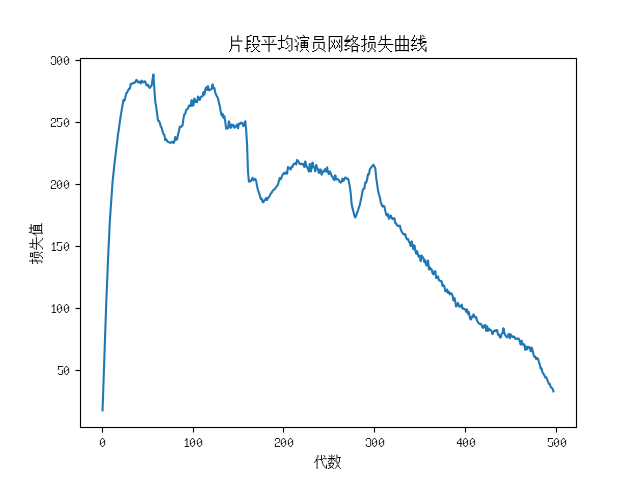
\includegraphics[width=0.6\textwidth]{mujoco_lossmu.png}
        \caption{$\mu$的损失曲线}
            \label{mujocolossmu}
        \end{figure}

        如图\ref{mujocolossmu}所示,演员网络在每个片段的平均损失在前60代快速上升,并在之后有回跳地下降。

        评论家网络1和评论家网络2的每个片段的平均损失如图\ref{mujocolossq1}和\ref{mujocolossq2}。
        通过对比可以看出两个图中的损失曲线的变化趋势大致相同且剧烈变化之处与演员网络的损失相似,这可能是由于评论家网络的好坏通过损失影响了演员网络表示的确定性策略的好坏。

        \begin{figure}[htpb]
        \centering
        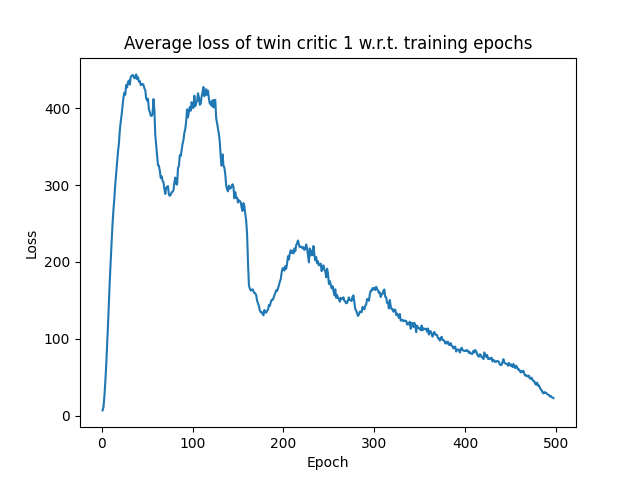
\includegraphics[width=0.6\textwidth]{mujoco_lossq1.png}
        \caption{$Q_1$的损失曲线}
        \label{mujocolossq1} 
        \end{figure}

        \begin{figure}[htpb]
        \centering
        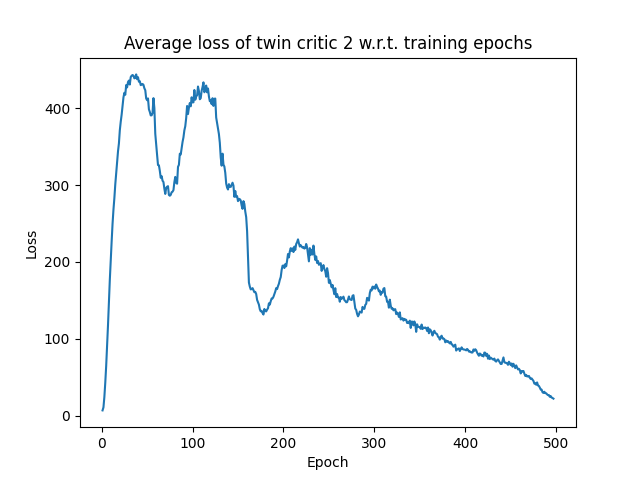
\includegraphics[width=0.6\textwidth]{mujoco_lossq2.png}
        \caption{$Q_2$的损失曲线}
        \label{mujocolossq2} 
        \end{figure}

        每一代(10个片段)的平均环境奖励如图\ref{mujocoreward}所示。
        可以看出,随着训练的片段数和代数增多,环境的奖励开始逐渐增大,最终达到-5左右。
        \begin{figure}[htpb]
        \centering
        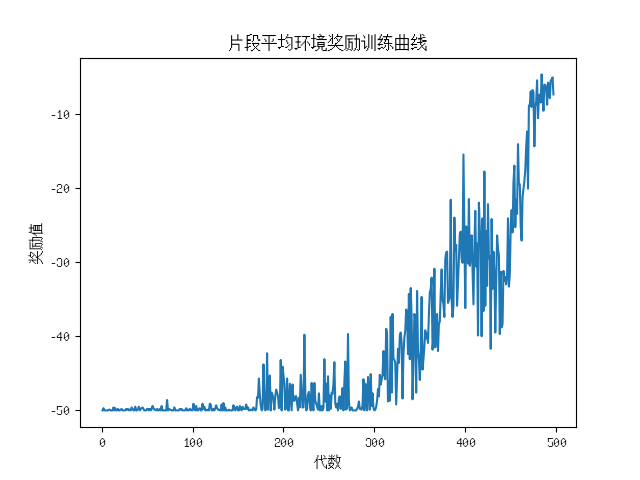
\includegraphics[width=0.6\textwidth]{mujoco_reward.png}
        \caption{环境奖励}
            \label{mujocoreward}
        \end{figure}

        平均每个片段的成功率如图\ref{mujocosuc}所示。
        每个片段的成功与否是通过片段末尾的奖励来判断的,若片段末尾的状态中的已完成的目标与期望目标的距离小于给定值,得到了值为0.0的奖励,就说这个片段成功完成了任务。由于成功率仅仅是10个片段的平均值得到的,因此它只能取到10个离散的值。
        因为成功率的计算只考虑了最后一个状态,所以成功率曲线与平均奖励曲线不完全相同。
        \begin{figure}[htpb]
        \centering
        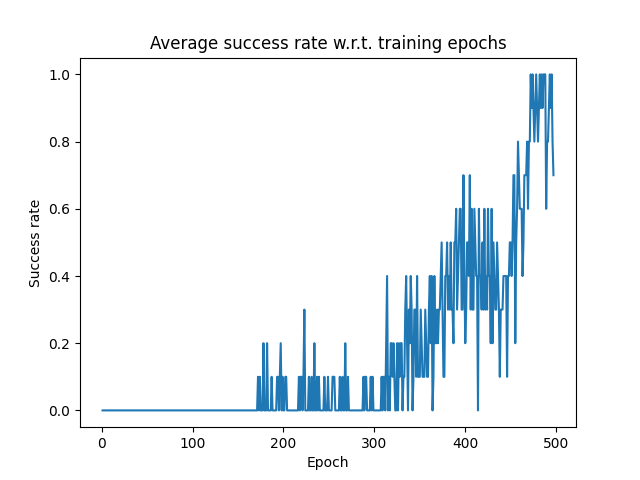
\includegraphics[width=0.6\textwidth]{mujoco_suc_rate.png}
        \caption{任务目标的平均成功率}
            \label{mujocosuc}
        \end{figure}

        在训练完成后,仿真环境\emph{FetchReach-v1}中的这个机械臂已经可以控制它的关节并快速地使末端执行器达到红点位置,成功率约为90\%。如图\ref{mujoco_gym}所示,机械臂成功地完成了任务.
        \begin{figure}[htpb]
        \centering
        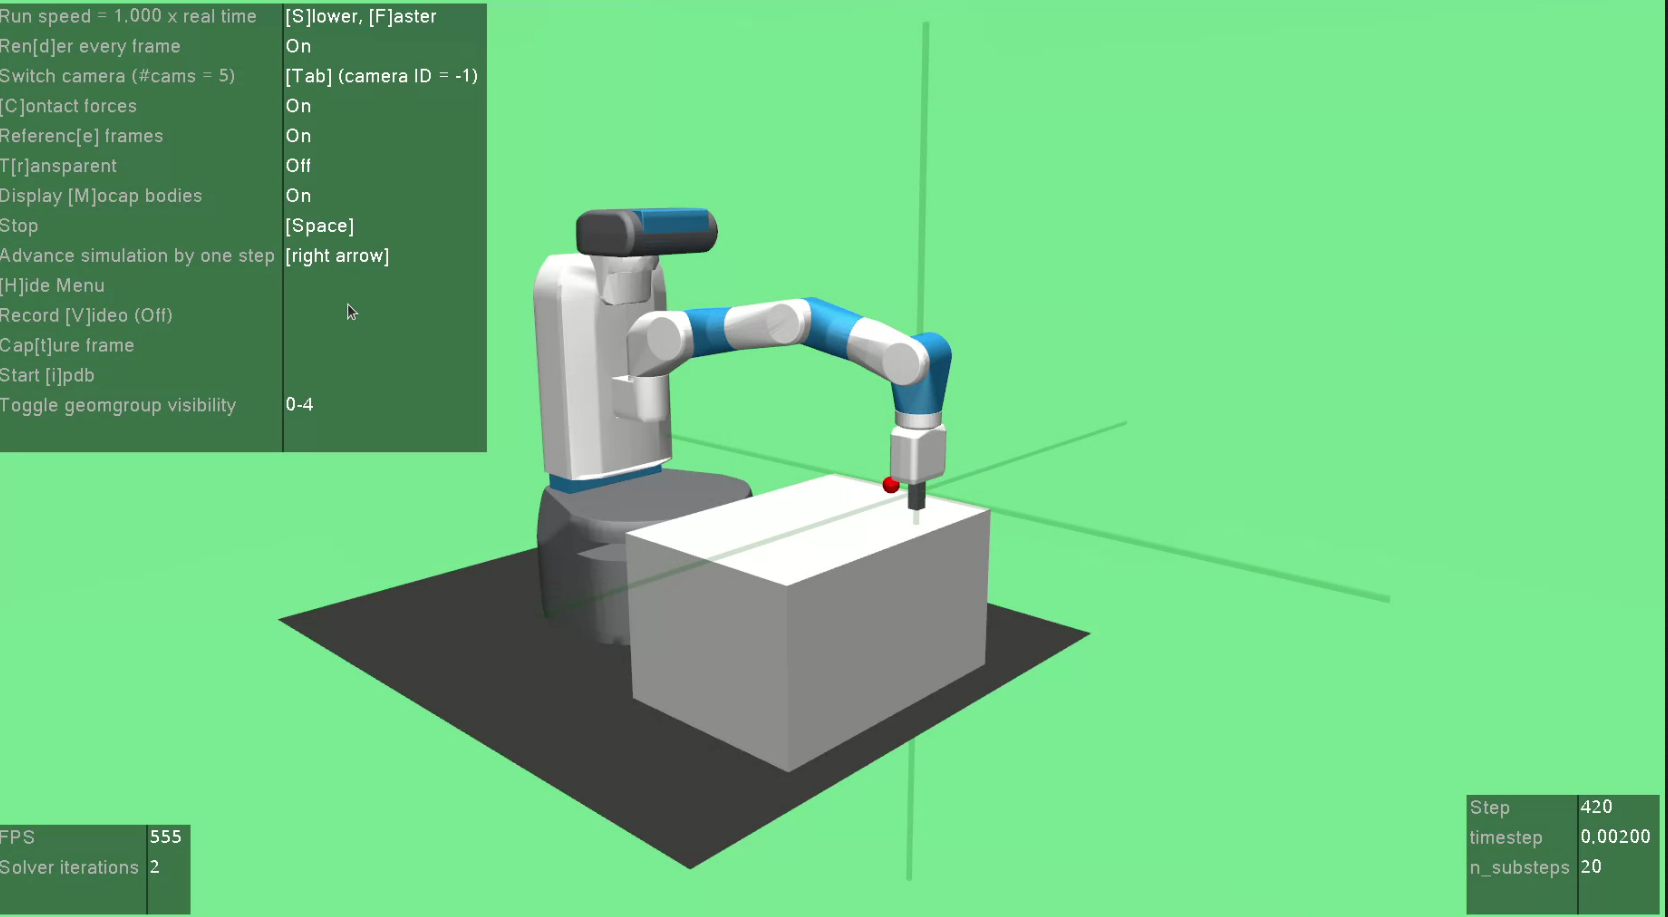
\includegraphics[width=0.8\textwidth]{mujoco_gym.png}
            \caption{机械臂完成任务的结果图。其中Fetch便携机械臂控制关节使末端执行器达到了红点位置,成功完成了指定任务目标。}
            \label{mujoco_gym}
        \end{figure}

        可以预见的是,由于对轨迹进行替换引入了大量重复的迁移,轨迹替换方法会比未来替换方法对针对稀疏奖励的强化学习加速的效果更差。
        但是,不同于未来替换方法,轨迹替换方法可以很好地适用于状态向量不显式包含已完成的目标和期望目标的环境。
        对于一条失败轨迹$(s_1,a_1,r_t,s_2),\cdots,(s_T,a_T,r_T,s_{T+1})$,可以将其视为一整个序列$D$,引入一个校正算法$\mathcal A:D\mapsto D'$,将状态和奖励进行替换,模拟一个更容易成功的轨迹。

        在开放任务中,已完成的目标和期望目标往往与其他状态变量相关,很难分离出来,但是对于一整个轨迹,可以控制动作序列不变,选择容易引起成功的环境初始化方法,对整个轨迹进行重新仿真和替换,相当于进行了后验的思考。
        对于一些任务,即使使用了未来替换策略,由于已完成的目标和期望目标并不包含与完成任务相关的信息,替换往往不会带来明显的收敛速度提升,但对于此类任务,轨迹替换方法仍然适用。
        因此,轨迹替换方法有更强的适用性,比未来替换方法更适合于状态变量关系复杂,难以分离或任务目标不包含有效信息的开放任务。


\section{混合高斯噪声层}

通常情况下,为了增加策略的稳健性,会对演员网络输出的动作向量添加一个均值为0,标准差为定值的高斯噪声。得到的动作常常还要进行裁剪以防止出现不合理的动作。然而,此种方法需要对两个超参数进行调节,需要大量的时间来进行训练,寻找最优的超参数值。由于在此主体实验中,往往需要训练很长的时间,因此引入这两个超参数并不理想。
    
为了避免手动调节噪声大小,本文提出了一个嵌入演员网络的可自动调节的混合高斯噪声。这个自动调节的噪声向量是通过直接在正态噪声向量后添加全连接层来得到的。得到的噪声向量被加到演员网络最后一层的输出上。
形式化地,给定一个从正态分布中随机采样的$B\times \mathrm{dim}(a)$的高斯噪声矩阵$X_{B\times \mathrm{dim}(a)}$,其中$B$是训练的迁移批次大小,$\mathrm{dim}(a)$是动作空间的维度大小。
如果把演员网络中确定性的部分的输出表示为$f(s)$,其中$s$是输入的状态向量,则有如下缩放后的噪声:

    $$ \mu(s) = f(s) + W X + b, X_{ij}\sim\mathcal N(0,1),$$

    其中$W$和$b$是全连接层的权重,它们通过反向传播自动调节。

    为了更好地展示添加此混合高斯噪声层的效果,研究中在Pyrobolearn中的自定义环境中进行了两个实验以进行对照。其中一个有着固定的噪声大小作为超参数,而另一个没有此超参数而是换成了本文提出的混合高斯噪声层。
    实验系统的基本设计已经在\ref{myenvexp}中进行了详细讨论。本实验中使用了\ref{td3sec}中描述的未来替换方法,与\ref{myenvexp}中不同的是,在这两个实验中对每个网络都多添加了一层隐藏层。此外,随机初始化时对蓝色方块使用了$x,y\in[-1,1]$的均匀采样,WAM机械臂的最后一个末端执行器与方块的距离达到0.5米以内即可获得0.0的奖励,其余情况获得-1.0的奖励,且对靶网络的更新每2个片段进行一次。使用的实验参数如表\ref{fcntable}所示,其中符号的意义与\ref{pretable}中相同。

    \begin{table}[htbp]
        \caption{混合高斯噪声层实验参数}
        \label{fcntable}
    \vspace{0.5em}\centering\wuhao
    \begin{tabular}{ccccc}
    \toprule[1.5pt]
    实验参数 & 值\\
    \midrule[1pt]
        $\epsilon_{noise}$ & 0.2\\
        $\sigma_{clip}$ & 0.5\\
        $M$ & $5\times 10^3$\\
        $\epsilon_{rand}$ & 0.3\\
        $\gamma$ & 0.991\\
        $\alpha$ & $3\times 10^{-4}$\\
        $B$ & 16\\
        $\tau$ & 0.005\\
        $T$ & 50\\
        $f_\mu$ & 2\\
        $T_{start}$ & $2.5\times 10^4$\\
        $N_{sample}$ & 200 \\
        $k$ & 18\\
        $K_{replay}$ & 4\\
        $\xi_{LSH}$ & $2\times 10^{-2}$\\
    \bottomrule[1.5pt]
    \end{tabular}
    \end{table}
    其中$k$是\ref{LSHsec}中的超参数,用于调整对状态空间离散化的粒度。
    $K_{replay}$是\ref{HERsec}中所述的超参数,它与替换掉的迁移的比例有关。
    $\xi_{LSH}$是在计算最终奖励时,基于局部敏感哈希和计数的探索奖励的系数。
    其余参数的意义与表\ref{pretable}中相同。

    平均每个片段的使用混合高斯噪声层的演员网络的损失和使用噪声大小超参数的演员网络的损失如图\ref{fcn_lossmu}所示。有混合高斯噪声层的演员网络的损失在较少的代数内上升到了一个相对较低的值。由于这两组实验中损失都收敛到了较高的值,此损失曲线并不能明确反映哪种方法更优,因为演员网络的损失是由评论家网络决定的,而这两组实验中的评论家并不一定具有相同权重,因此即使是相同的演员网络也有可能具有不同的损失。

        \begin{figure}[htpb]
        \centering
        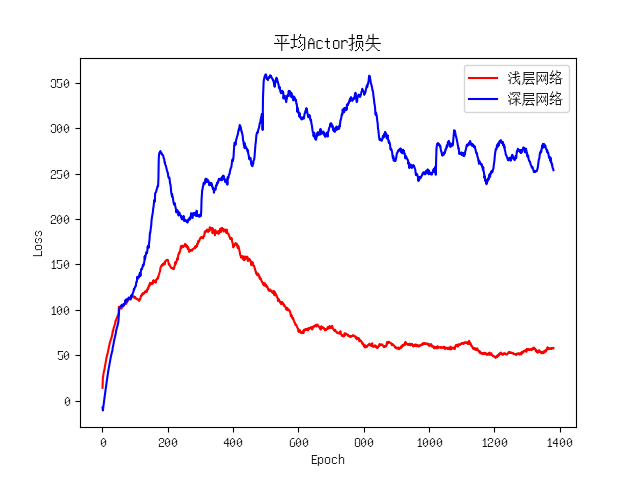
\includegraphics[width=0.6\textwidth]{myenv_lossmu.png}
        \caption{演员网络$\mu$的损失曲线}
            \label{fcn_lossmu}
        \end{figure}

    每个片段的评论家网络$Q_1$和$Q_2$的平均损失分别如图\ref{fcn_lossq1}和图\ref{fcn_lossq2}所示。可以看出,它们的损失也是和演员网络$\mu$的损失具有相似的形状。由于评论家网络的损失也并没有收敛到较低的值,这些损失曲线也不能反映混合高斯噪声层带来的变化。但是可以肯定的是,添加混合高斯噪声层后损失曲线变化更加平缓了。从图中也可以看出,评论家网络的损失比演员网络的损失更加不稳定,这可能是由于评论家网络的损失直接与环境相关导致的。

        \begin{figure}[htpb]
        \centering
        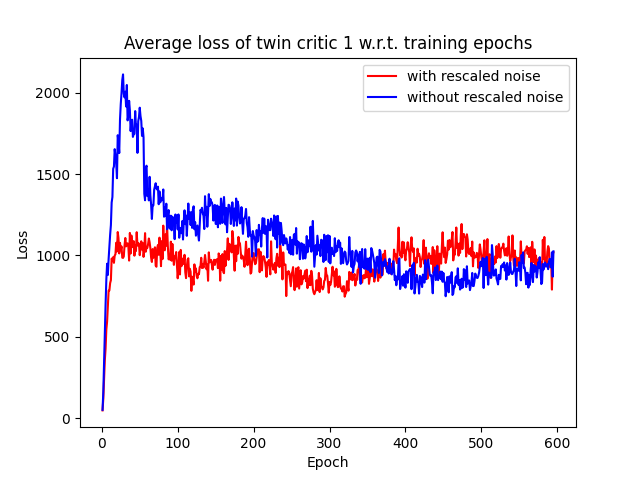
\includegraphics[width=0.6\textwidth]{myenv_lossq1.png}
        \caption{评论家网络$Q_1$的损失曲线}
            \label{fcn_lossq1}
        \end{figure}

        \begin{figure}[htpb]
        \centering
        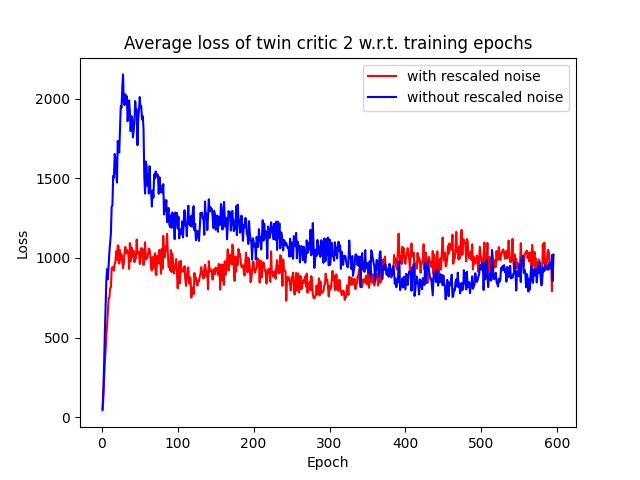
\includegraphics[width=0.6\textwidth]{myenv_lossq2.png}
        \caption{评论家网络$Q_2$的损失曲线}
            \label{fcn_lossq2}
        \end{figure}

        使用和不使用混合高斯噪声层的单位片段平均环境奖励如图\ref{fcn_reward}所示。可以看出,添加了混合高斯噪声层的方法获得的奖励要稍微比只使用噪声大小超参数的方法更高。

        \begin{figure}[htpb]
        \centering
        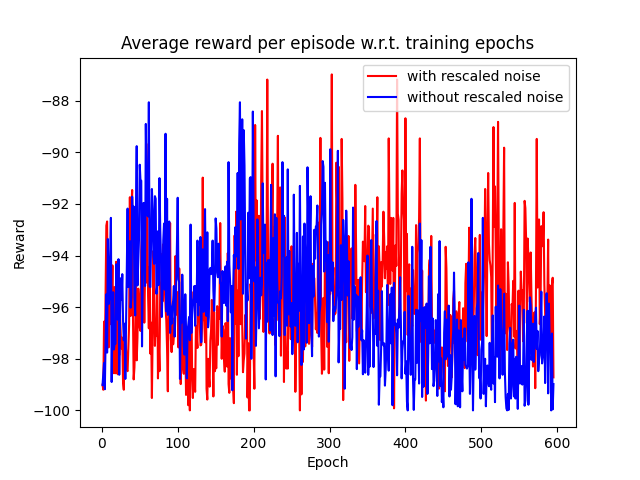
\includegraphics[width=0.6\textwidth]{myenv_reward.png}
        \caption{平均环境奖励曲线}
            \label{fcn_reward}
        \end{figure}

        平均成功率曲线的变化趋势与平均环境奖励的大致相同。对于最后的平均成功率,添加了混合高斯噪声层的要稍微更高。

        \begin{figure}[htpb]
        \centering
        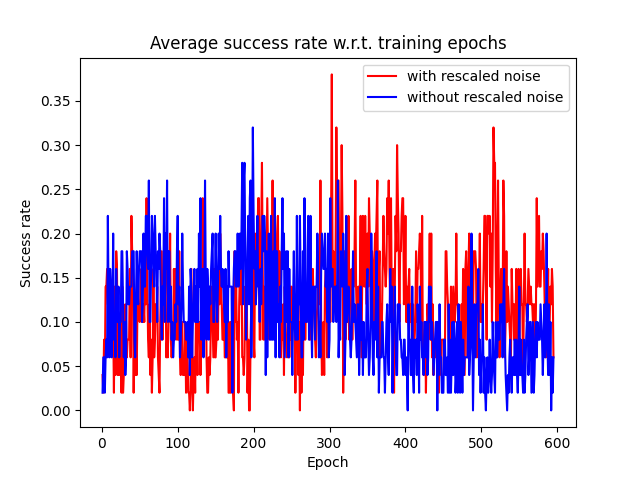
\includegraphics[width=0.6\textwidth]{myenv_suc_rate.png}
        \caption{任务目标成功率}
            \label{fcn_suc_rate}
        \end{figure}

        在引入混合高斯噪声层之后,本研究中使用的TD3算法实际上由确定性策略梯度算法转化为了非确定性策略梯度算法。
        混合高斯噪声层通过自适应地调整噪声向量的大小和方向,可以更好地适应开放任务中复杂的动力学过程,更好地探索低概率的动作,防止策略收敛到局部最优,并加速算法的收敛。


\section{仿真时间奖励}

在对物理过程进行仿真的过程中,物理引擎往往会做一些缓存和优化来对仿真进行加速,而这种加速是基于此物理过程容易预测这一事实的。这意味着,对于难以进行预测的复杂物理行为,如复杂的碰撞,物理引擎要消耗更多的时间来进行仿真。这就使得利用此信息来为智能体提供任务无关的探索奖励成为可能。

在实验过程中,为了准确计算仿真时间,避免其他因素影响,必须保证在训练过程中没有其他程序在运行。这一要求可以简单地通过避免在训练时操作计算机来满足。此外,为了防止系统调用的时间被计入,在实验中对仿真时间进行计算时,直接在仿真代码被调用前后使用Python的time库进行了计时。

除了仿真时间奖励外,实验中还提供了基于局部敏感哈希的探索奖励。为了平衡不同的内部奖励,需要在计算最终奖励前先乘上一个系数。

在演员网络中,使用了上一章提出的混合高斯噪声层,但不同的是,为了防止噪声产生过大影响,继续使用参数$\sigma_{clip}$对噪声进行裁剪。

为了防止机械臂在可以完成任务的动作序列中选择较长的序列,在对演员网络进行优化时,可以在其损失函数中添加一个动作惩罚项,即

   $$ L_\mu = -\sum_i^N\frac{Q_1(s_i, \mu(s_i))}{N} + \xi_{action}||\mu(s_i)||^2$$
其中$\xi_{action}$是动作惩罚系数。

在时间步$t$的仿真时间奖励计算及相关过程如算法\ref{simtimereward}所示,在使用演员网络$\mu$获得下一步动作后,使用$Time$函数获得当前时间,执行动作并仿真后再获得当前时间,将时间差作为仿真时间奖励。
其中$Random$是生成[0,1]均匀分布的随机数的函数,$RandomAction$是生成随机动作的函数,$Env$表示环境对智能体动作的响应,重放缓冲$B_{replay}$被用于保存每一个时间步中由仿真时间奖励和基于局部敏感哈希的计数奖励构成的内部奖励$r^{in}_t$和相关的动作和状态。
在需要对演员网络和评论家网络进行训练时,只需从重放缓冲中采样保存的迁移$(s_t,a_t,r_t,s_{t+1})$,并根据事后经验重放算法对其中一些状态进行替换并计算环境奖励,与内部奖励求和后构成用于训练的迁移。
\begin{algorithm}
    \AlgoBiCaption{仿真时间奖励\label{simtimereward}}{Simulation Time Reward}
    \KwIn{状态$s_t$}
    \KwOut{仿真时间奖励$r^{sim}_t$,重放缓冲$B_{replay}$}

    \If{$Random()<\epsilon_{rand}$}{$a_t=\mu(s_t)$}
    \Else{$a_t=RandomAction()$}
    $t_1 = Time()$\\
    $s_{t+1}=Env(a_t)$,即在环境中执行动作$a_t$并使用仿真器仿真\\
    $t_2 = Time()$\\
    $r^{sim}_t=\xi_{sim}(t_2-t_1)$\\
    $r^{lsh}_t=reward_{lsh}(s_t)$\\
    $r^{in}_t=r^{sim}+r^{lsh}$\\
    将$s_t,a_t,r^{in}_t,s_{t+1}$加入重放缓冲$B_{replay}$中
\end{algorithm}


在实验中,整个系统都采用\ref{myenvexp}中的设计,但是除了使用\ref{myenvexp}中的浅层网络结构外,还增加了一个为每个网络添加一个隐藏层的深层网络作为对照组。

实验相关的参数见表\ref{simtable}。
    \begin{table}[htbp]
        \caption{仿真时间奖励实验参数}
        \label{simtable}
    \vspace{0.5em}\centering\wuhao
    \begin{tabular}{ccccc}
    \toprule[1.5pt]
    实验参数 & 值\\
    \midrule[1pt]
        $\sigma_{clip}$ & 0.5\\
        $M$ & 300\\
        $\epsilon_{rand}$ & 0.3\\
        $\xi_{action}$ & $1\times 10^{-3}$\\
        $\gamma$ & 0.998\\
        $\alpha$ & $1\times 10^{-3}$\\
        $B$ & 10000\\
        $\tau$ & 0.23\\
        $T$ & 200\\
        $N_{batches}$ & 1\\
        $f_{target}$ & 200\\
        $f_{actor}$ & 400\\
        $f_{critic}$ & 200\\
        $T_{start}$ & $1\times 10^5$\\
        $N_{sample}$ & 50 \\
        $k$ & 18\\
        $K_{replay}$ & 4\\
        $\xi_{LSH}$ & $2\times 10^{-2}$\\
        $\xi_{sim}$ & 10\\
    \bottomrule[1.5pt]
    \end{tabular}
    \end{table}
    其中$\xi_{action}$是动作惩罚系数,$N_{batches}$指每次触发对演员网络或评论家网络的训练时迭代的次数。
    每经过$f_{target}$个时间步,使用指数滑动平均对靶网络进行权重更新。
    每经过$f_{actor}$个时间步,使用反向传播对演员网络权重进行更新。
    每经过$f_{critic}$个时间步,使用优化器对评论家网络权重进行更新。
    $\xi_{sim}$是在计算最终奖励时,仿真时间奖励的系数。
    其余的参数意义与表\ref{fcntable}中相同。

只有3层与有4层的网络相比,演员网络损失曲线如图\ref{simlossmu}所示。可以看出浅层网络更快地收敛了,而深层网络收敛到了一个损失较大的值。
        \begin{figure}[htpb]
        \centering
        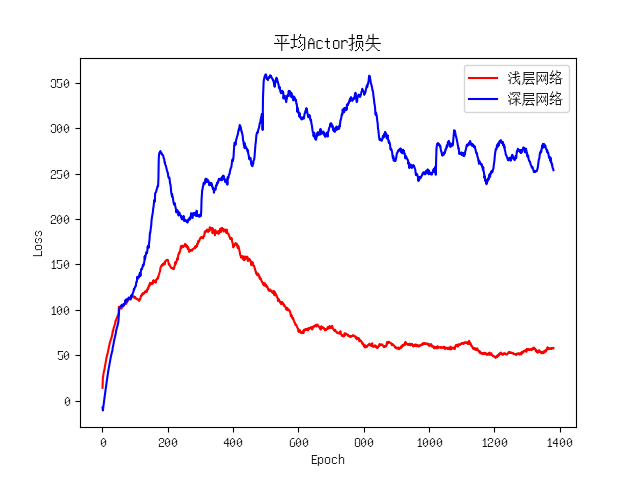
\includegraphics[width=0.6\textwidth]{sim_myenv_lossmu.png}
        \caption{3层和4层演员网络$\mu$的损失曲线}
            \label{simlossmu}
        \end{figure}

对于评论家网络来说,如图\ref{simlossq1}和\ref{simlossq2}所示,情况是类似的,更加值得注意的是,深层网络更容易出现损失突然暴增的现象,这意味着深层网络训练起来更加不稳定。
        \begin{figure}[htpb]
        \centering
        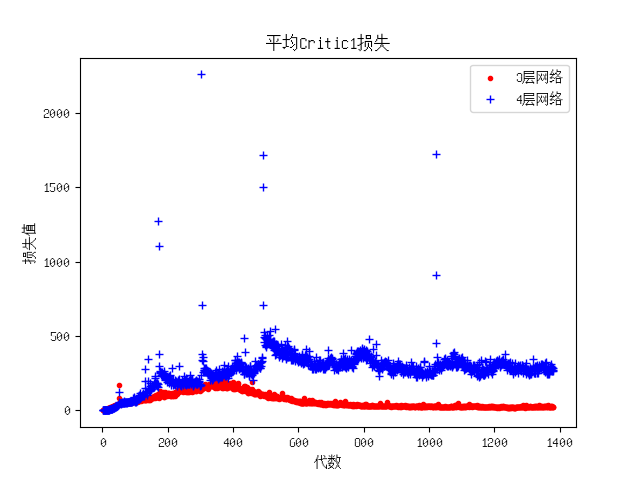
\includegraphics[width=0.6\textwidth]{sim_myenv_lossq1.png}
        \caption{3层和4层评论家网络$Q_1$的损失曲线}
            \label{simlossq1}
        \end{figure}

        \begin{figure}[htpb]
        \centering
        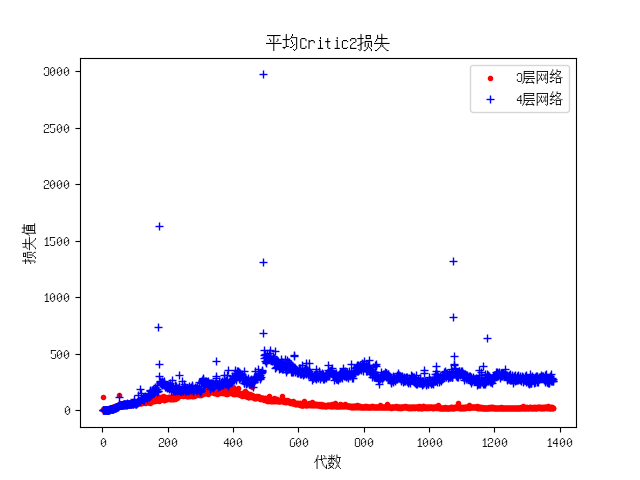
\includegraphics[width=0.6\textwidth]{sim_myenv_lossq2.png}
        \caption{3层和4层评论家网络$Q_2$的损失曲线}
            \label{simlossq2}
        \end{figure}

浅层网络和深层网络的平均环境奖励如图\ref{simenv_reward}所示,可以看出浅层最后学习到了一个较好的策略,得到的奖励显著比深层网络更高,而深层网络的奖励一直维持在最差的结果附近。

        \begin{figure}[htpb]
        \centering
        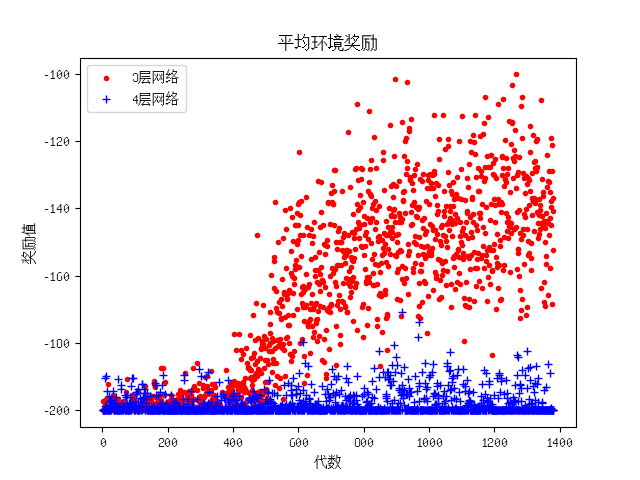
\includegraphics[width=0.6\textwidth]{sim_myenv_reward.png}
        \caption{浅层神经网络和深层神经网络的平均环境奖励曲线}
            \label{simenv_reward}
        \end{figure}

观察图\ref{simlsh_reward}中所示的基于局部敏感哈希的计数奖励可以发现,浅层网络的基于局部敏感哈希的计数奖励与深层网络的相差不多,甚至在200代附近深层网络反而获得了更高的奖励。

        \begin{figure}[htpb]
        \centering
        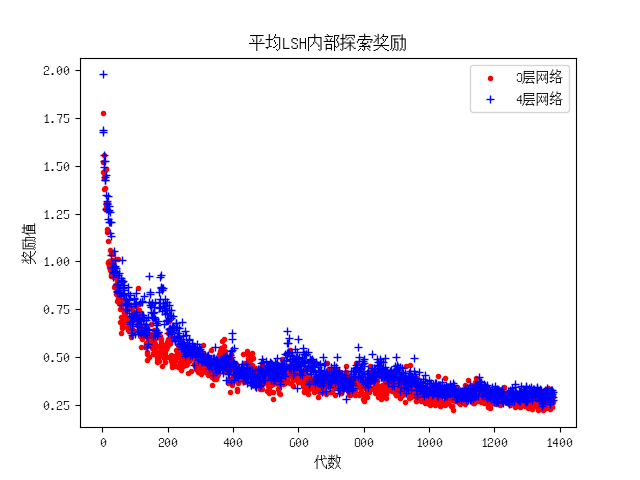
\includegraphics[width=0.6\textwidth]{sim_myenv_lsh_reward.png}
        \caption{浅层网络和深层网络的基于局部敏感哈希的平均计数奖励曲线}
            \label{simlsh_reward}
        \end{figure}
而仿真时间奖励则能比基于局部敏感哈希的计数奖励更好地反映策略的好坏,如图\ref{simsim_reward}所示,仿真时间奖励在900代之后浅层网络要比深层网络更高,这与环境奖励的趋势吻合,表明仿真时间奖励不仅具有任务无关的鼓励智能体探索的能力,还能帮助智能体在探索之后策略泛化到给定开放任务中。

        \begin{figure}[htpb]
        \centering
        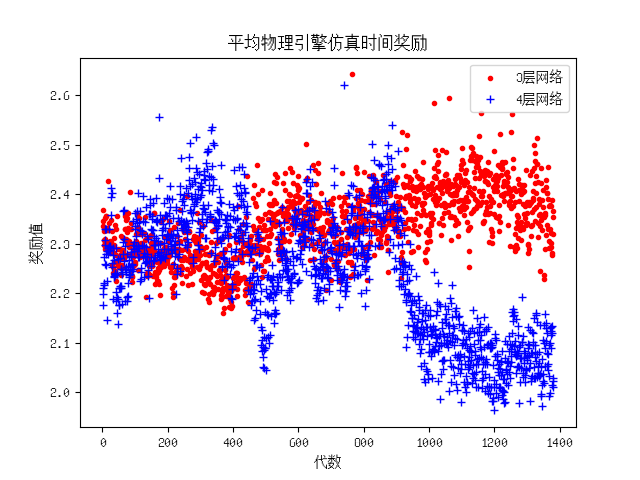
\includegraphics[width=0.6\textwidth]{sim_myenv_sim_reward.png}
        \caption{浅层网络和深层网络的平均仿真时间奖励曲线}
            \label{simsim_reward}
        \end{figure}
图\ref{simsuc_rate}中的成功率变化与环境奖励的变化趋势相似,这和在其他实验中观察到的一致。

        \begin{figure}[htpb]
        \centering
        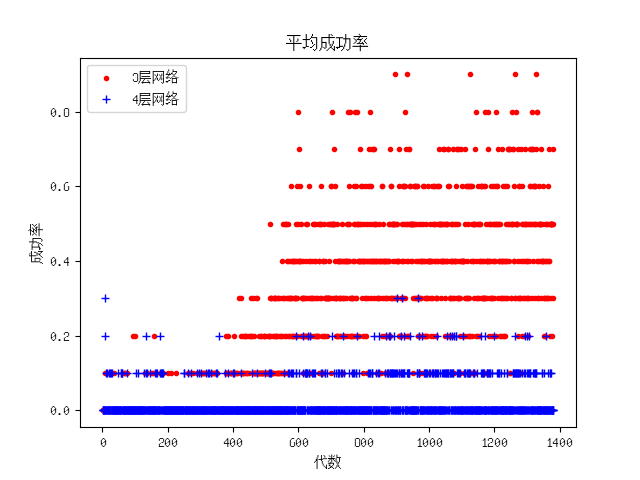
\includegraphics[width=0.6\textwidth]{sim_myenv_suc_rate.png}
        \caption{浅层网络和深层网络平均任务目标成功率曲线}
            \label{simsuc_rate}
        \end{figure}
实验中在对深层网络的梯度进行观测时,发现演员网络中的梯度快速地减小至0,这意味着发生了梯度消失,如果使用残差网络、层归一化或进行谱归一化,则有可能进一步提高性能。

在训练完成后,智能体完成接近方块的开放任务的成功率约为60\%,如图\ref{reach}所示为智能体成功完成任务时的截图。

        \begin{figure}[htpb]
        \centering
        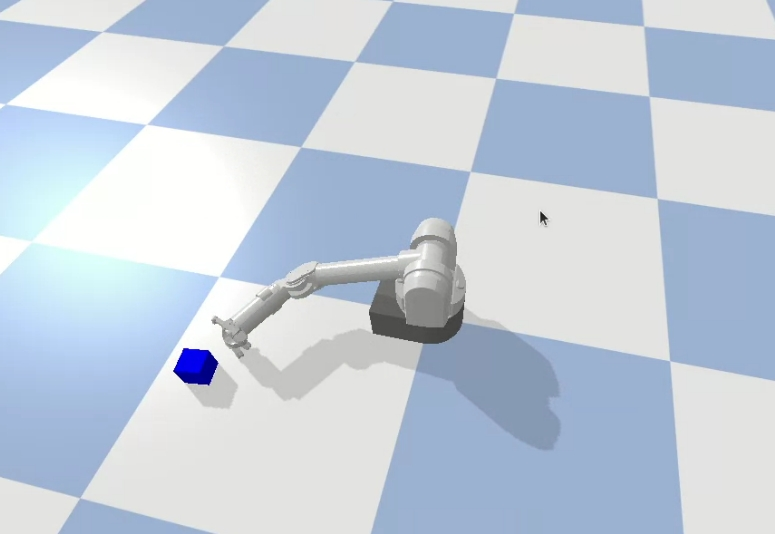
\includegraphics[width=0.6\textwidth]{reach.jpg}
        \caption{机械臂智能体完成任务的结果展示}
            \label{reach}
        \end{figure}
仿真时间奖励可以适用于几乎所有的基于物理引擎的强化学习环境。
由于仿真时间的获取非常容易,几乎不需要额外开销,这使得智能体的训练速度几乎不受影响。
在开放任务中,任务的完成往往要经过复杂的动力学过程,如碰撞、摩擦等过程,而且这些过程的仿真需要更长的时间,因此仿真时间奖励可以很好地应用于此种类型的开放任务,并通过利用此先验知识在环境中探索获得更好的元探索策略。
\section{本章小结}
本章针对开放任务特点提出了轨迹替换方法、混合高斯噪声层和仿真时间奖励。

轨迹替换方法针对开放任务中已完成的目标和期望目标有时难以提供有效信息或难以从状态变量中分离的特点,提出了对整个轨迹使用一定方法进行替换,具有更强的适用性。

混合高斯噪声层针对开放任务中一些动作难以取到的问题,通过对固定动作噪声进行改进,可以获得更快的收敛速度和更好的探索策略。

仿真时间奖励针对任务完成过程涉及复杂动力学过程的开放任务,将仿真时间开销作为奖励,鼓励智能体探索更复杂的动力学过程。
它可以作为内部奖励加速开放任务算法收敛速度,也可以作为元探索策略帮助智能体在环境中探索。
